\subsubsection{Расположения файлов мессенджера Viber}
 
В зависимости от операционной системы (в дальнейшем ОС) у Viber разные пути установки. Для Windows XP: C:\textbackslash Documents and Settings\textbackslash \%Username\%\textbackslash Application Data\textbackslash ViberPC.
Для Windows 7, 8, 8.1, 10: C:\textbackslash Users\textbackslash \%Username\%\textbackslash AppData\textbackslash Roaming\textbackslash ViberPC (рис.~\ref{kucher_1:kucher_1}).
 
\begin{figure}[h!]
\center{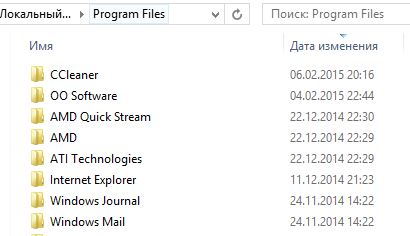
\includegraphics[width=0.8\linewidth]{kucher_1}}
\caption{ Путь к файлам Viber }
\label{kucher_1:kucher_1}
\end{figure}

\subsubsection{Описание содержимого папки «ViberPC»}

При изучении содержимого папки «ViberPC» было обнаружено, что интересующая информация содержится в папках, название которых – номер телефона (рис.~\ref{kucher_2:kucher_2}).
	

\begin{figure}[h!]
\center{
\includegraphics[width=0.8\linewidth]{kucher_2}}
\caption{ Содержимое папки с номером телефона }
\label{kucher_2:kucher_2}
\end{figure} 

\begin{itemize}
  \item Папка «Avatars» – содержит изображения пользователей;
  \item Папка «Thumbnails» – содержит все изображения, которые были отправлены и получены в ходе переписки;
	«viber.db» – база данных (далее БД), в которой хранится информация о контактах, переписках, звонках.
	БД «viber.db» – имеет формат SQLite format 3 (рис.~\ref{kucher_3:kucher_3}).
\end{itemize}
 
\begin{figure}[h!]
\center{
\includegraphics[width=0.3\linewidth]{kucher_3}}
\caption{ Содержимое БД «viber.db» }
\label{kucher_3:kucher_3}
\end{figure} 

\subsubsection{SQL-запросы для получения информации}

Чтобы получить все контакты и их имена был написан следующий SQL-запрос: 
\textit{Select ContactRelation.Number, Contact.FirstName from СontactRelation, Contact where Contact.ContactID = ContactRelation.ContactID}.

Чтобы получить все контакты и имена, на которые можно позвонить в Viber, нужен следующий SQL-запрос: 
\textit{Select Contact.FirstName, ContactRelation.Number from contact, PhoneNumber, ContactRelation where PhoneNumber.IsViberNumber = 1 and PhoneNumber.Number = ContactRelation.Number and ContactRelation.ContactID = Contact.ContactID}.

Чтобы связать изображение пользователя с номером телефона и именем, нужен следующий SQL-запрос:
\textit{Select Contact.FirstName, ContactRelation.Number, OriginNumberInfo.AvatarPath From OriginNumberInfo, ContactRelation, Contact Where OriginNumberInfo.Number = ContactRelation.Number and ContactRelation.ContactID = Contact.ContactID}.

Для получения информации о звонках которые осуществлялись через Viber, нужен следующий запрос: 
\textit{select Contact.FirstName, Events.Direction, datetime(Events.TimeStamp, 'unixepoch') from Contact, Events, ContactRelation where Events.EventID = (select Calls.EventID from Calls) AND Events.Number = ContactRelation.Number and ContactRelation.ContactID = Contact.ContactID}.

Для получения текста переписки с конкретным пользователем нужно знать его номер чата. Для получения всех номеров чата нужно воспользоваться следующим запросом: 
\textit{Select ChatInfo.ChatID, Contact.FirstName, ChatInfo.TokenFrom ChatInfo, ContactRelation, Contactwhere ChatInfo.Token = ContactRelation.Number and ContactRelation.ContactID = Contact.ContactID}.

Зная номер чата, можно получить текст переписки: 
\textit{select Messages.Body, Contact.FirstName, Events.Direction, Messages.ThumbnailPath, datetime(Events.TimeStamp, 'unixepoch') from messages, Events, Contact, ContactRelation where Messages.EventID = Events.EventID and Events.Number = ContactRelation.Number and ContactRelation.ContactID = Contact.ContactID and Events.ChatID = @nomer\_chata}.

\subsubsection{Описание плагина}

Плагин «TaskViber» получает точку монтирования жесткого диска, с которого, в отличии от ОС, проверяет папку «ViberPC» у всех пользователей в ОС. Если папка «ViberPC» существует, то плагин извлекает информацию из аккаунтов, под которыми авторизовались с данного компьютера. Всю найденную информацию плагин сохраняет по указанному пути программного обеспечения «COEX». В папку «Avatars» (рис.~\ref{kucher_9:kucher_9}) копируются все найденные изображения пользователей. В папку «Thumbnails» (рис.~\ref{kucher_10:kucher_10}) копируются все изображения, которые были отправлены и получены в ходе переписки. В файле «Avatar Path.txt» находятся связи между изображениями пользователей, именами и номерами телефонов. В файле «Calls.txt» находятся описание звонков, которые осуществлялись через «Viber» (с кем был звонок, во сколько и кто кому звонил). В файле «Phone book.txt» находятся все номера телефонов и имена с мобильного телефона, на котором был зарегистрирован аккаунт в «Viber». В файле «Viber book.txt» находятся все номера телефонов и имена, которым можно позвонить через «Viber». В файле «Имя/номер messages.txt» содержится переписка с пользователем «Имя/номер» (с кем велась переписка, кто кому писал, что писал и во сколько писал).

Алгоритм работы плагина «TaskViber» представлен на рисунке~\ref{kucher_4:kucher_4}, алгоритм функции WinXP --- на рисунке~\ref{kucher_5:kucher_5}. Ниже также представлены алгоритмы работы Win\_7\_8\_10 (рис.~\ref{kucher_6:kucher_6}) и Viber\_XP\_7\_8\_10 (рис.~\ref{kucher_7:kucher_7}).

Результат работы плагина представлен на рисунке~\ref{kucher_8:kucher_8}.
 

\begin{figure}[h!]
\center{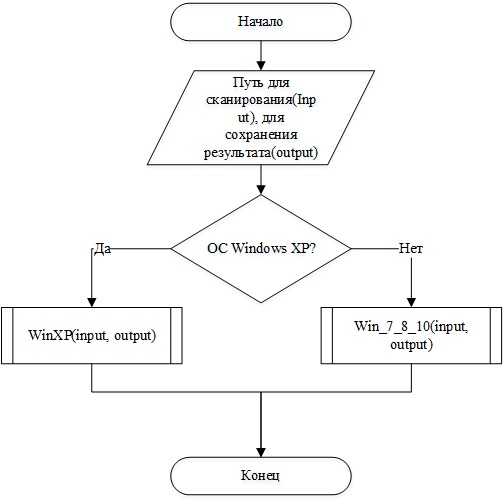
\includegraphics[width=0.6\linewidth]{kucher_4}}
\caption{ Алгоритм работы плагина }
\label{kucher_4:kucher_4}
\end{figure} 
  
\begin{figure}[h!]
\center{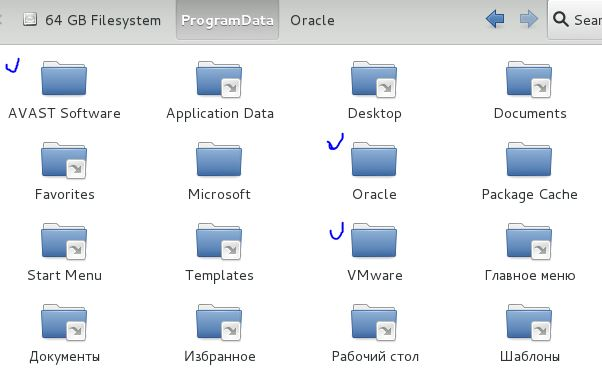
\includegraphics[width=0.6\linewidth]{kucher_5}}
\caption{ Алгоритм работы функции WinXP }
\label{kucher_5:kucher_5}
\end{figure} 

\begin{figure}[ht]
\center{
\includegraphics[width=0.6\linewidth]{kucher_6}}
\caption{ Алгоритм работы Win\_7\_8\_10 }
\label{kucher_6:kucher_6}
\end{figure} 

\begin{figure}[h!]
\center{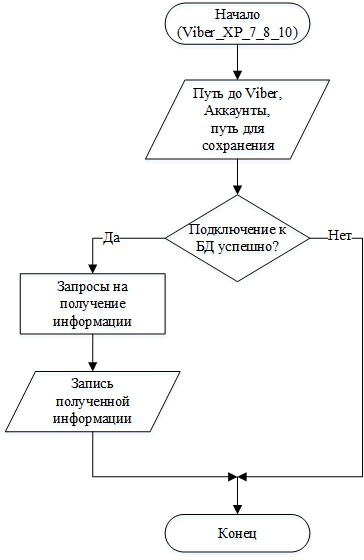
\includegraphics[width=0.5\linewidth]{kucher_7}}
\caption{ Алгоритм работы Viber\_XP\_7\_8\_10 }
\label{kucher_7:kucher_7}
\end{figure} 

\clearpage

\begin{figure}[h!]
\center{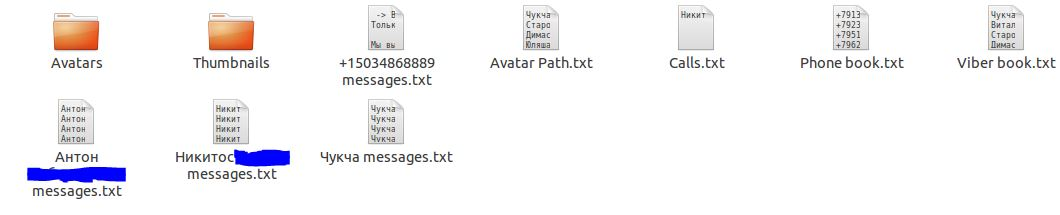
\includegraphics[width=1\linewidth]{kucher_8}}
\caption{ Результат работы плагина }
\label{kucher_8:kucher_8}
\end{figure} 

\begin{figure}[h!]
\center{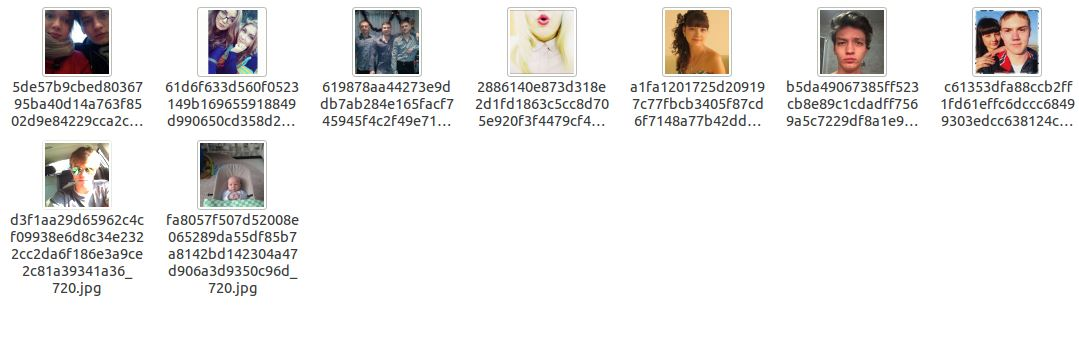
\includegraphics[width=1\linewidth]{kucher_9}}
\caption{ Содержимое папки «Avatars» }
\label{kucher_9:kucher_9}
\end{figure} 

\begin{figure}[h!]
\center{
\includegraphics[width=0.8\linewidth]{kucher_10}}
\caption{ Содержимое папки «Thumbnails» }
\label{kucher_10:kucher_10}
\end{figure} 

\clearpage
